\clearpage
\pagebreak

\subsection{Semester planning}

\begin{figure}[htb]
\begin{center}
\leavevmode
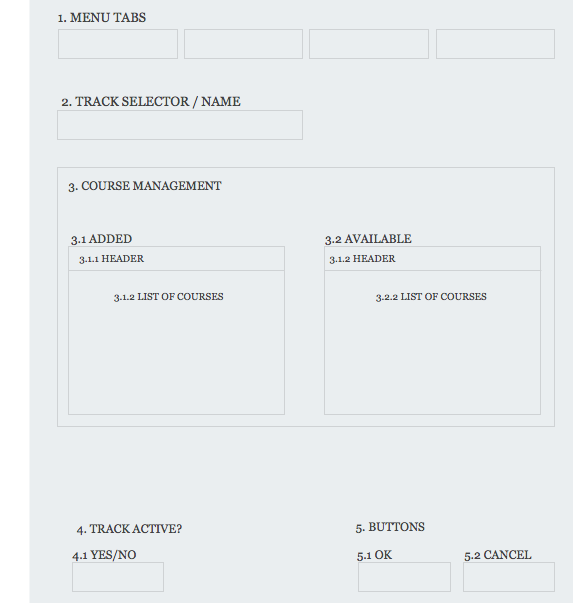
\includegraphics[width=0.75\textwidth]{images/wireframe_courses}
\end{center}
\caption{Wireframe for screen to add a course to the semester plan}
\label{fig:app2_mock1_w}
\end{figure}

\begin{figure}[htb]
\begin{center}
\leavevmode
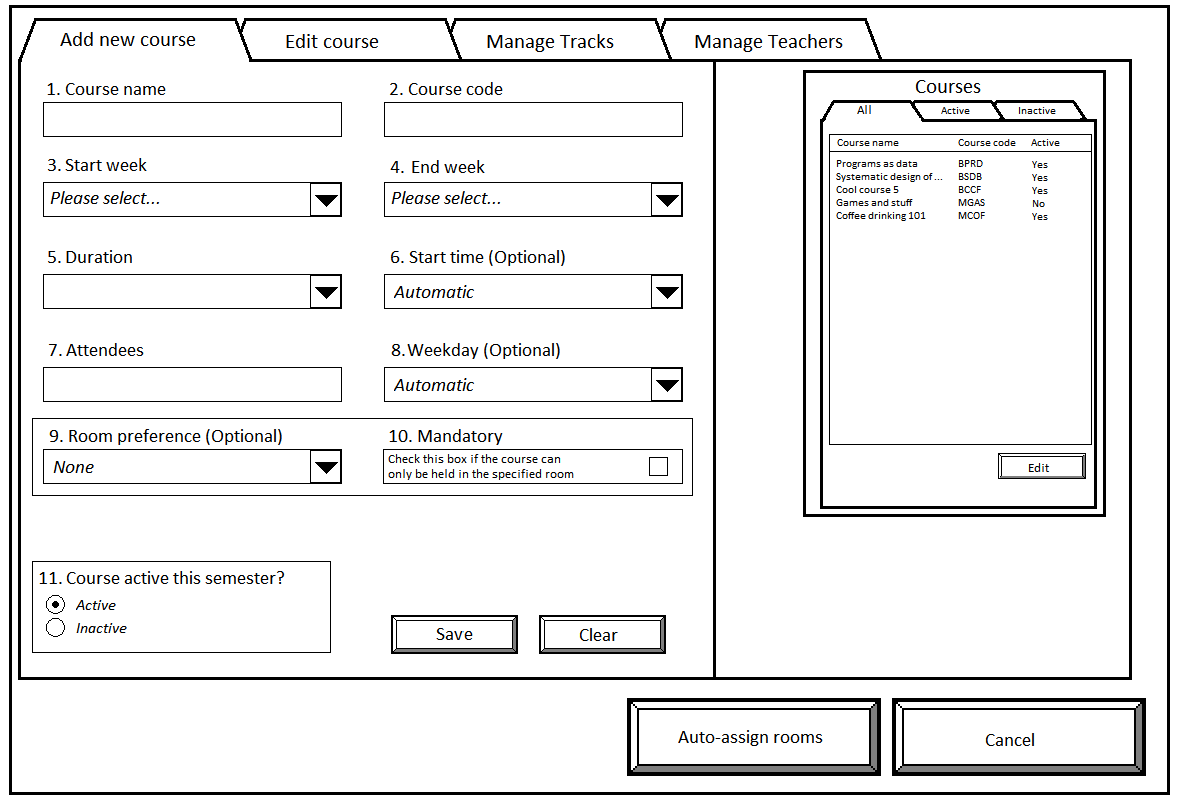
\includegraphics[width=0.75\textwidth]{images/courseplan2_addcourse}
\end{center}
\caption{Second mockup for screen to add a course to the semester plan}
\label{fig:app2_mock2_1}
\end{figure}

\begin{figure}[htb]
\begin{center}
\leavevmode
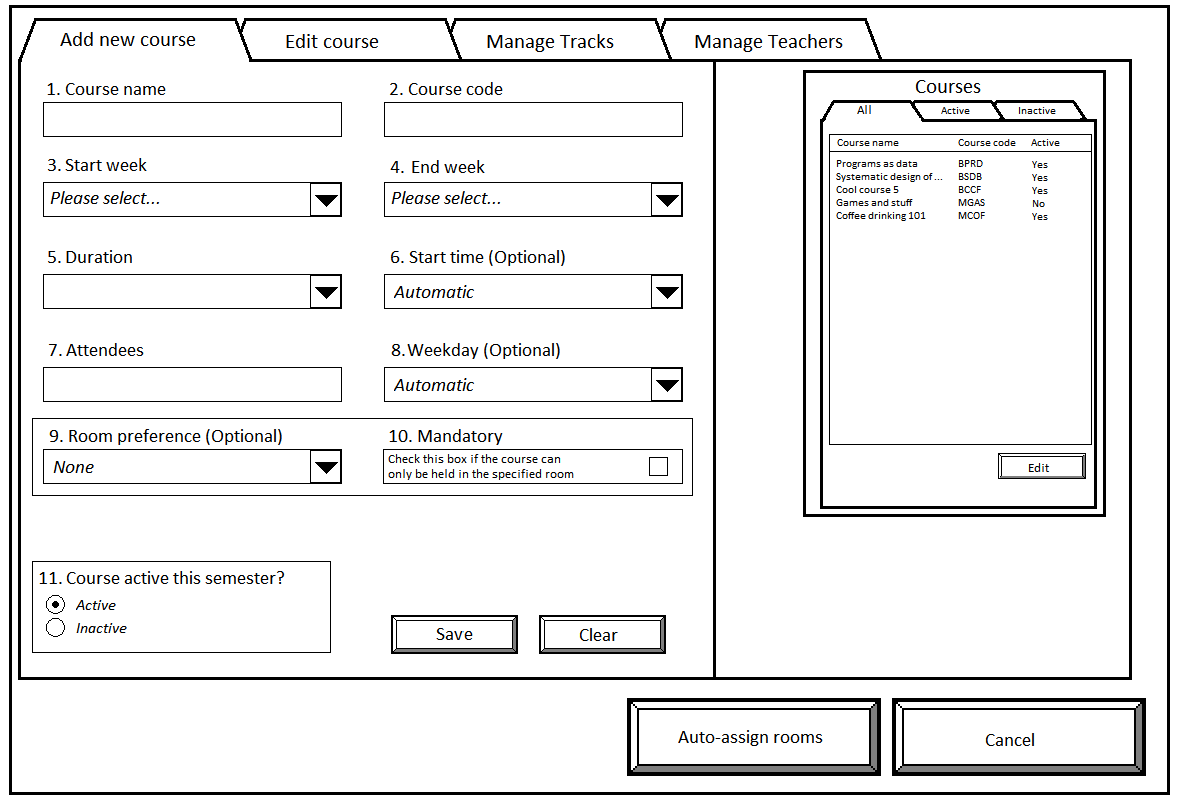
\includegraphics[width=0.75\textwidth]{images/courseplan2_addcourse}
\end{center}
\caption{Second mockup for screen to add a course to the semester plan}
\label{fig:app2_mock2_1}
\end{figure}

\begin{figure}[htb]
\begin{center}
\leavevmode
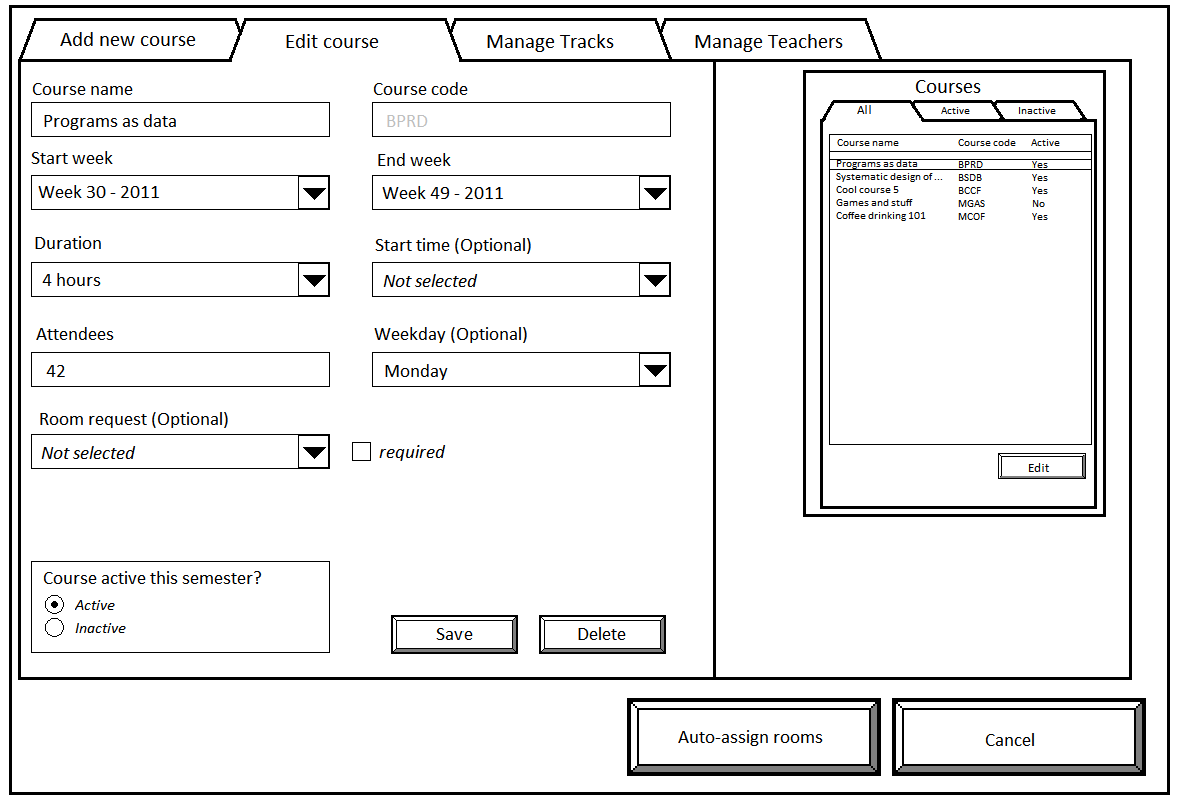
\includegraphics[width=0.75\textwidth]{images/courseplan_editcourse}
\end{center}
\caption{First mockup for screen to edit a course to the semester plan}
\label{fig:app2_mock1_2}
\end{figure}

\begin{figure}[htb]
\begin{center}
\leavevmode
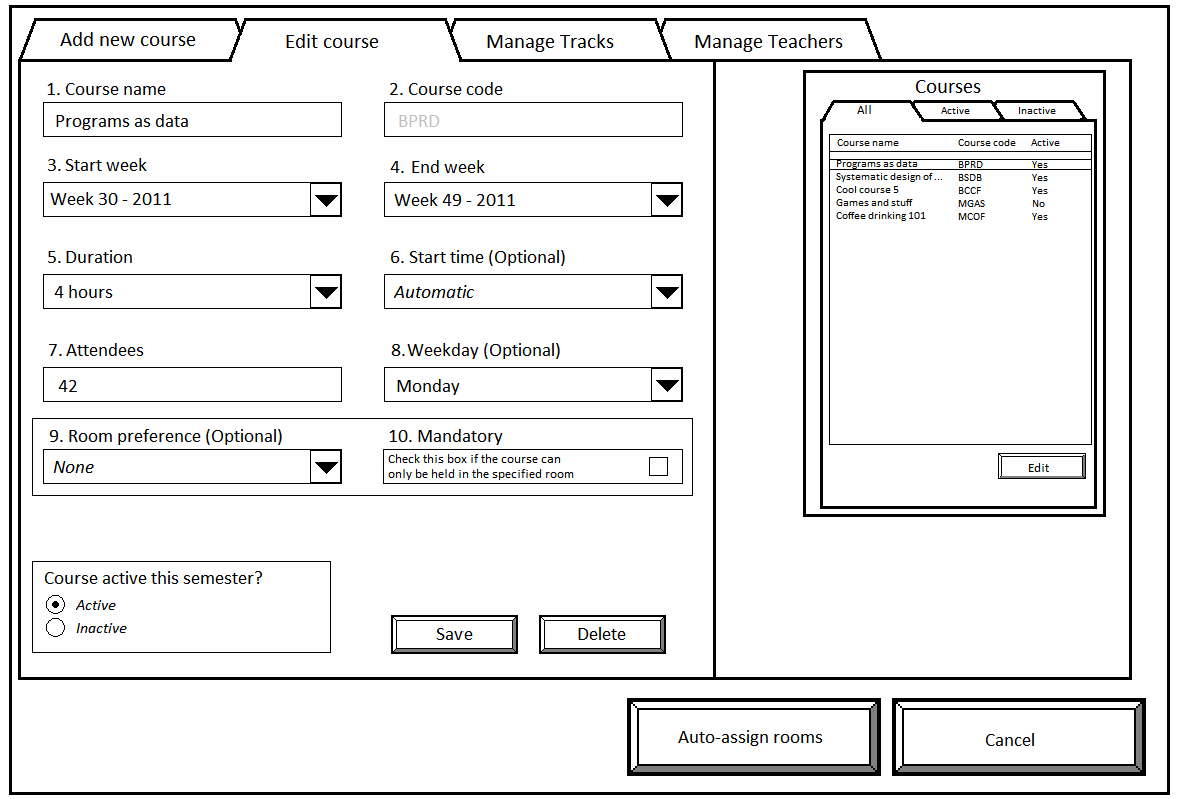
\includegraphics[width=0.75\textwidth]{images/courseplan2_editcourse}
\end{center}
\caption{Second mockup for screen to edit a course to the semester plan}
\label{fig:app2_mock2_2}
\end{figure}

\clearpage

\begin{figure}[htb]
\begin{center}
\leavevmode
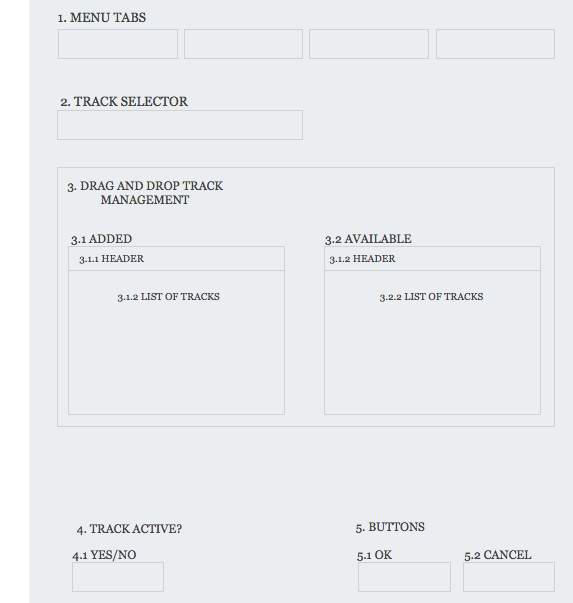
\includegraphics[width=0.75\textwidth]{images/wireframe_tracks}
\end{center}
\caption{Wireframe for screen to assign courses to tracks. (manage tracks)}
\label{fig:app2_mock1_w}
\end{figure}

\begin{figure}[htb]
\begin{center}
\leavevmode
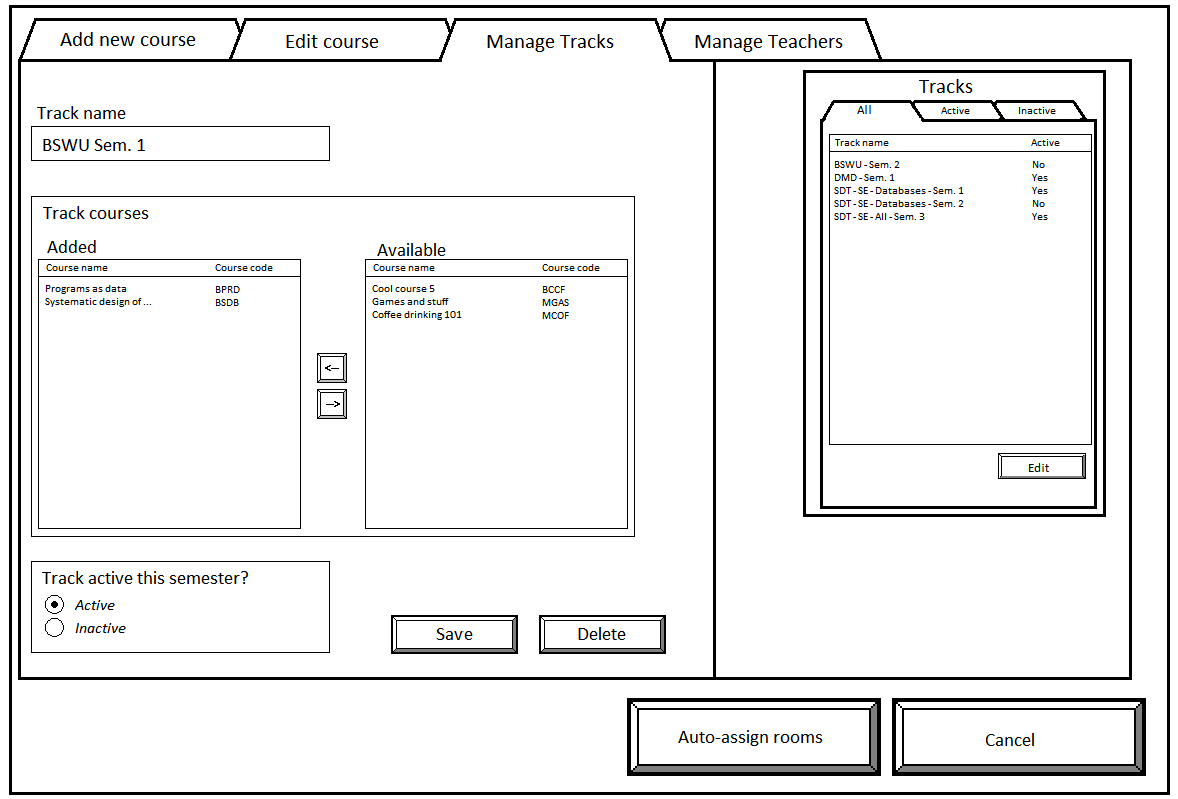
\includegraphics[width=0.75\textwidth]{images/courseplan_managetracks}
\end{center}
\caption{First mockup for screen to assign courses to tracks. (manage tracks)}
\label{fig:app2_mock1_3}
\end{figure}

\begin{figure}[htb]
\begin{center}
\leavevmode
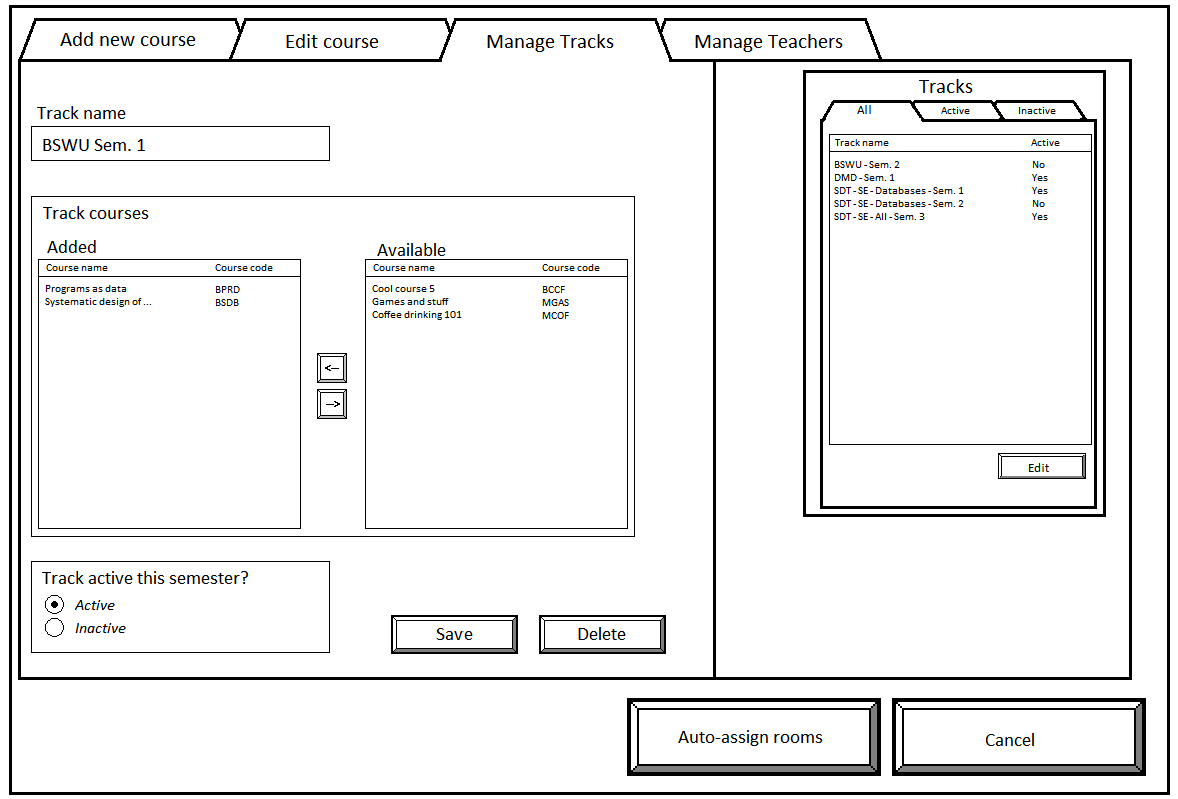
\includegraphics[width=0.75\textwidth]{images/courseplan2_managetracks}
\end{center}
\caption{Second mockup for screen to assign courses to tracks. (manage tracks)}
\label{fig:app2_mock2_3}
\end{figure}

\begin{figure}[htb]
\begin{center}
\leavevmode
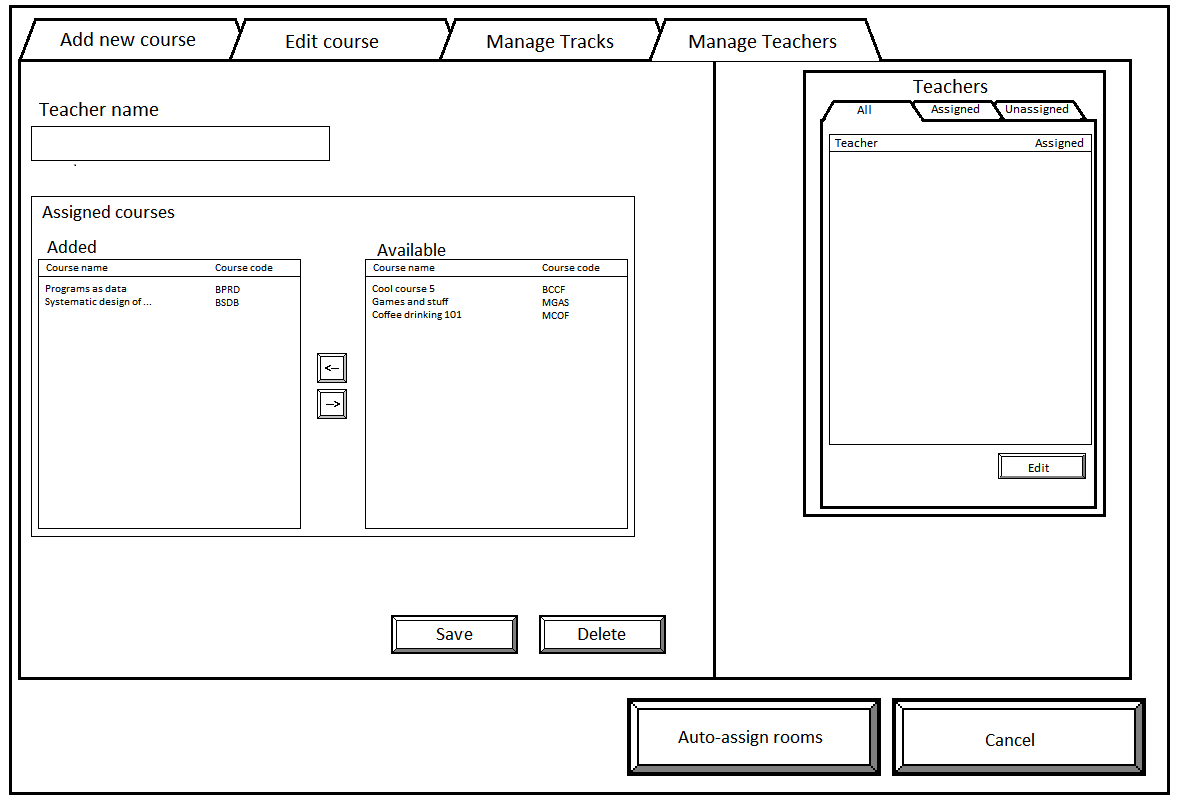
\includegraphics[width=0.75\textwidth]{images/courseplan_manageteachers}
\end{center}
\caption{First mockup for screen to assign teachers to courses. (manage teachers)}
\label{fig:app2_mock1_4}
\end{figure}

\begin{figure}[htb]
\begin{center}
\leavevmode
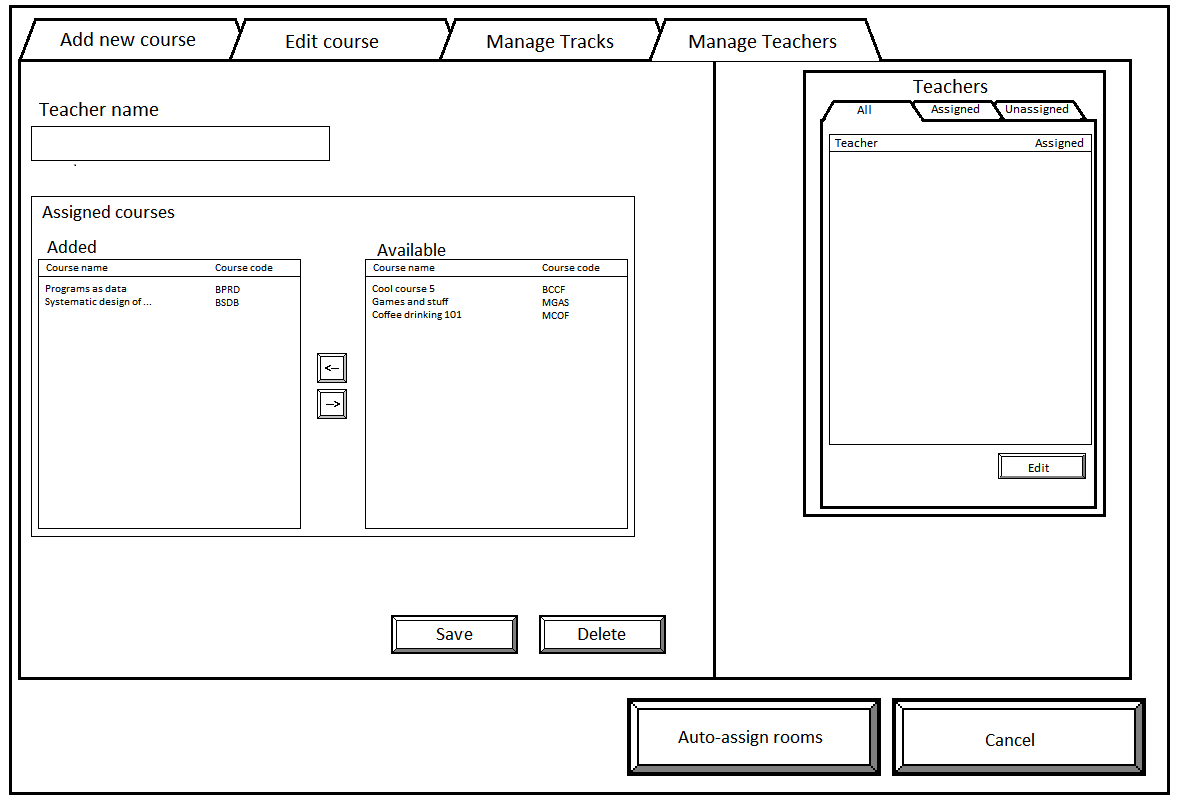
\includegraphics[width=0.75\textwidth]{images/courseplan2_manageteachers}
\end{center}
\caption{Second mockup for screen to assign teachers to courses. (manage teachers)}
\label{fig:app2_mock2_4}
\end{figure}

\begin{figure}[htb]
\begin{center}
\leavevmode
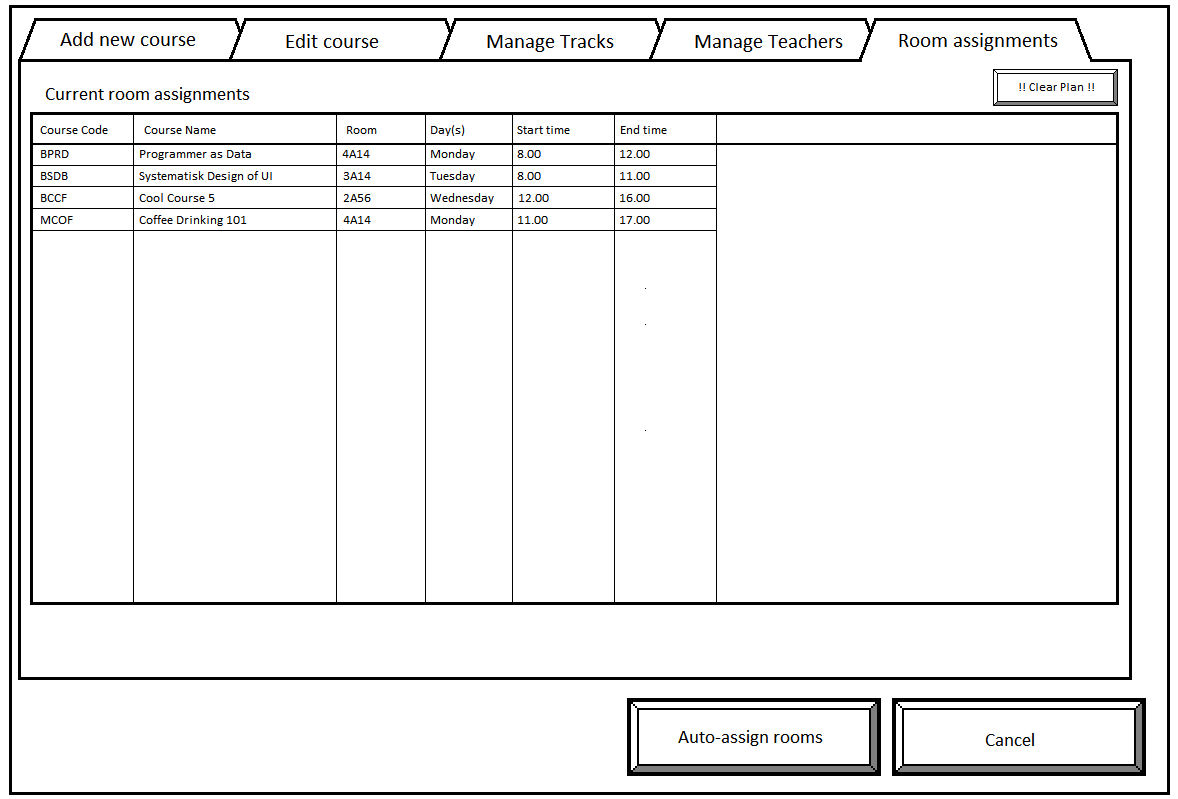
\includegraphics[width=0.75\textwidth]{images/courseplan_Room_Assignments}
\end{center}
\caption{First mockup for the screen showing the finished semester plan}
\label{fig:app2_mock1_5}
\end{figure}

\begin{figure}[htb]
\begin{center}
\leavevmode
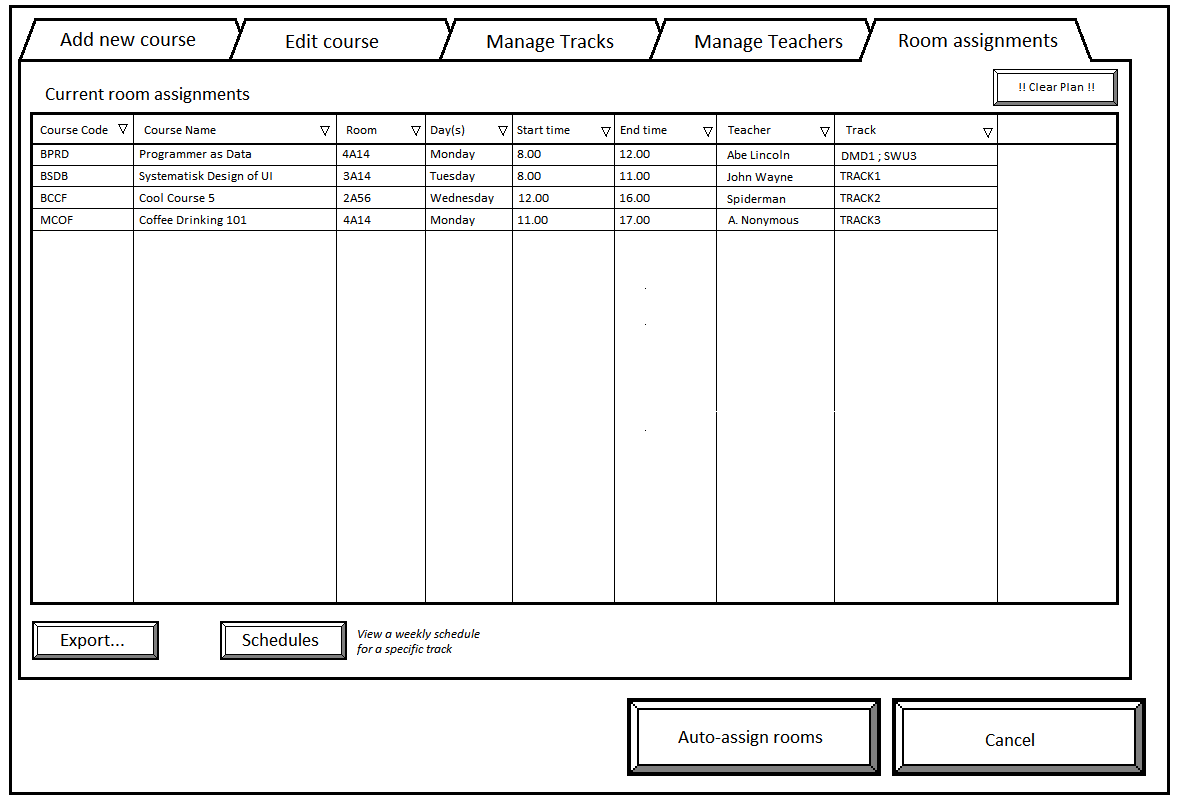
\includegraphics[width=0.75\textwidth]{images/courseplan2_Room_Assignments}
\end{center}
\caption{Second mockup for the screen showing the finished semester plan}
\label{fig:app2_mock2_5}
\end{figure}

\begin{figure}[htb]
\begin{center}
\leavevmode
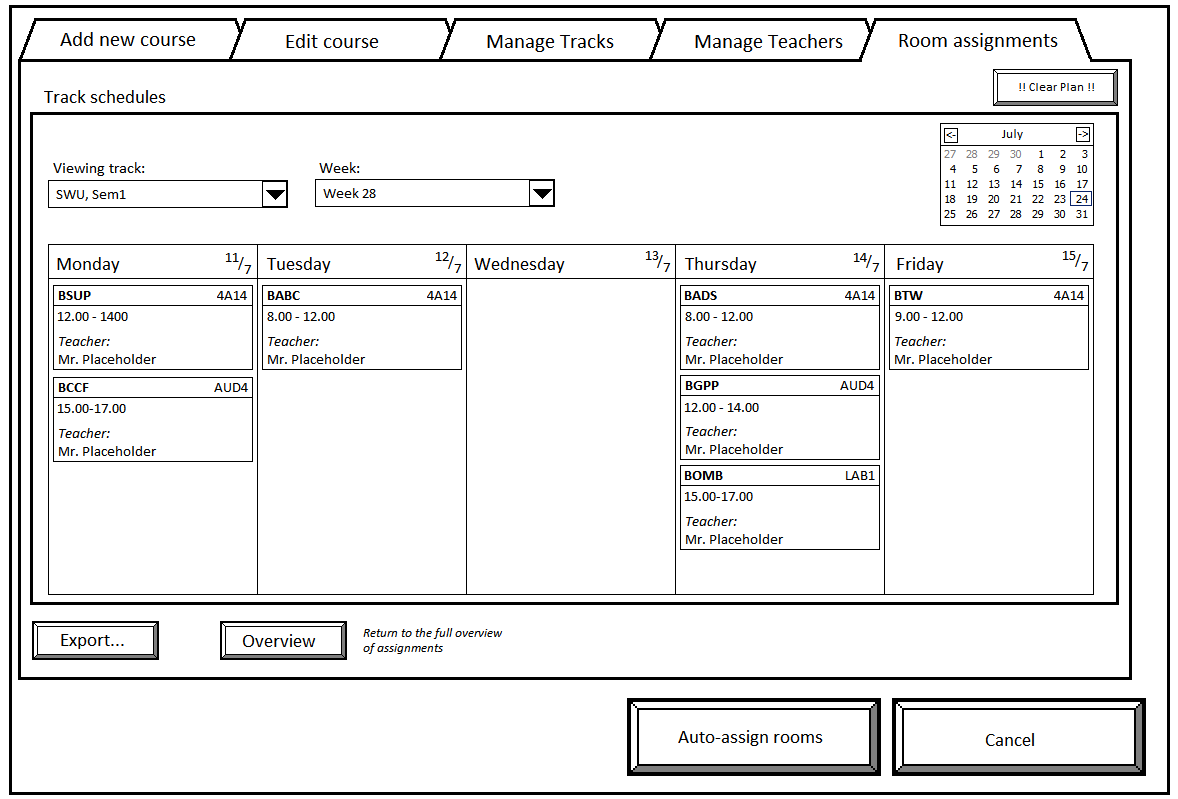
\includegraphics[width=0.75\textwidth]{images/courseplan2_Room_Assignments_schedules}
\end{center}
\caption{Mockup for the weekly schedule overview}
\label{fig:app2_mock2_6}
\end{figure}

\begin{figure}[htb]
\begin{center}
\leavevmode
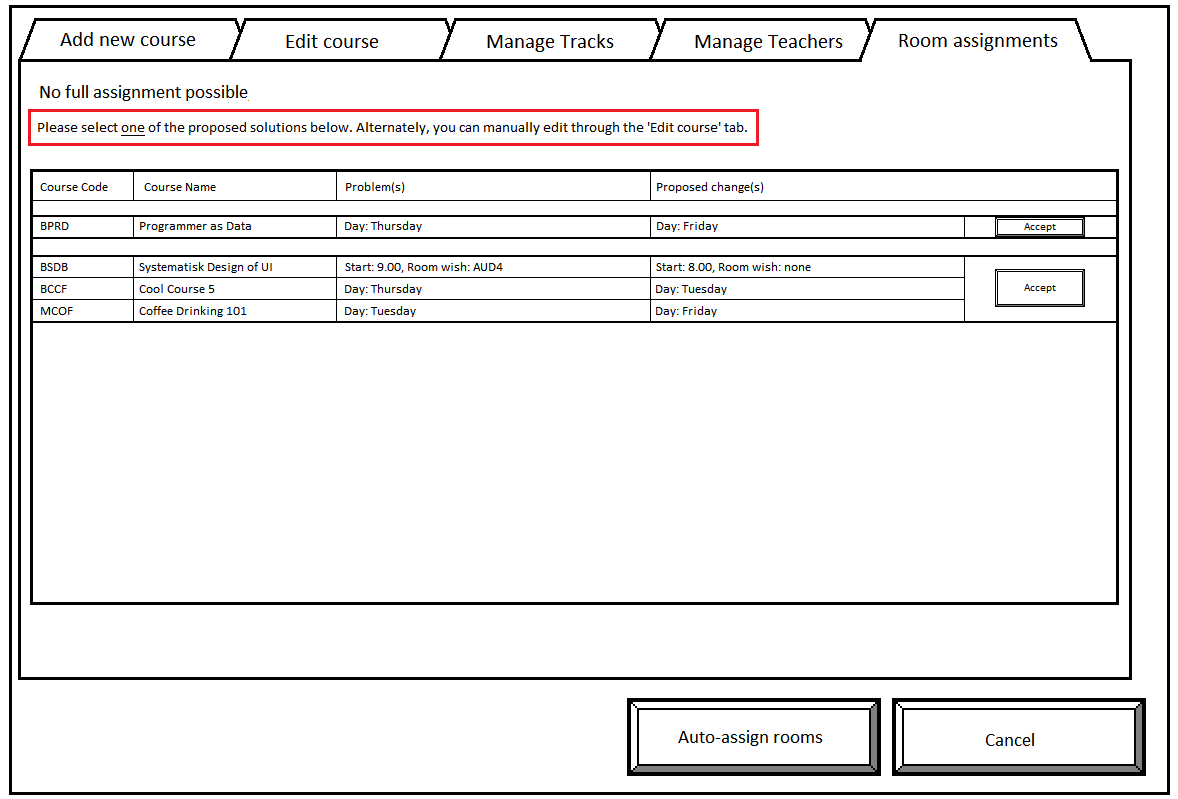
\includegraphics[width=0.75\textwidth]{images/courseplan_Room_Assignments_clash}
\end{center}
\caption{First mockup for the screen showing the finished semester plan, where some complications are present}
\label{fig:app2_mock1_7}
\end{figure}

\begin{figure}[htb]
\begin{center}
\leavevmode
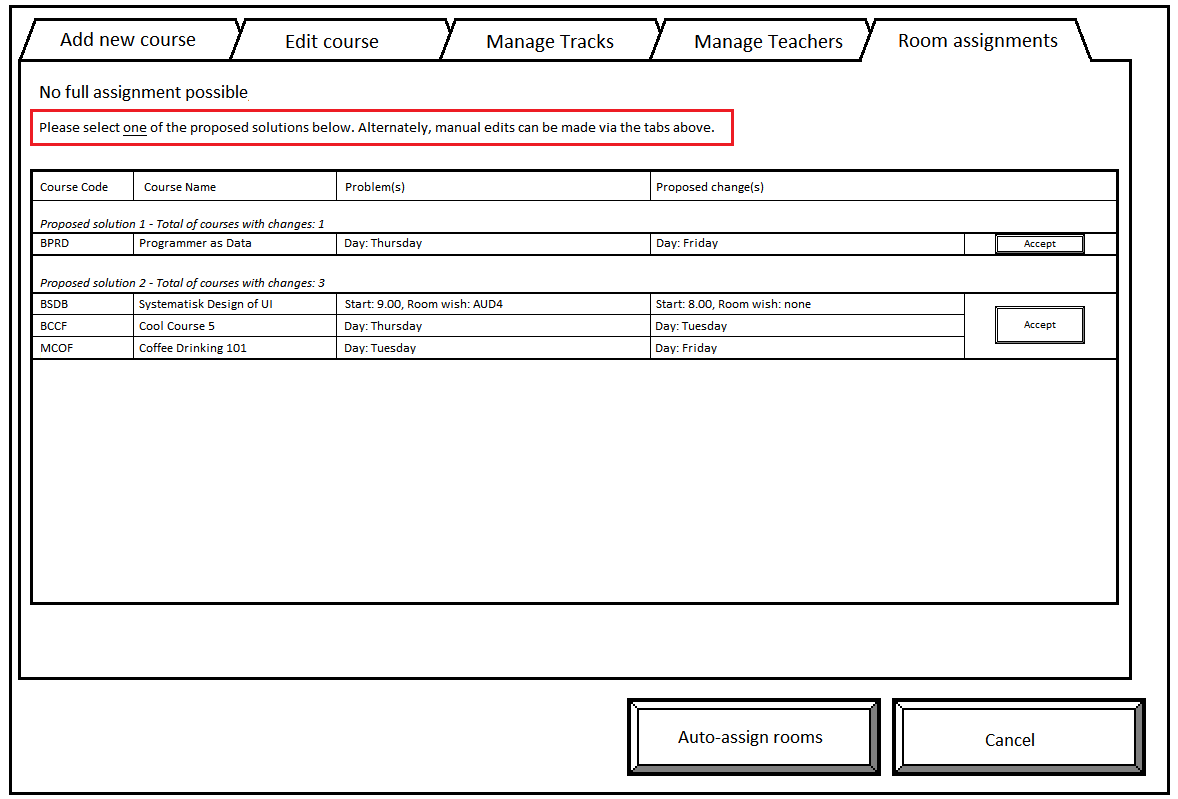
\includegraphics[width=0.75\textwidth]{images/courseplan2_Room_Assignments_clash}
\end{center}
\caption{Second mockup for the screen showing the finished semester plan, where some complications are present}
\label{fig:app2_mock2_7}
\end{figure}

\clearpage